\chapter{Estado del Arte} \label{cap:Estado del Arte} % chapter 3
%\section{Estado del Arte} \label{s:estado}
%\setcounter{section}{3}

En este capítulo explicaremos varios de los algoritmos SLAM más significativos, como MonoSLAM, PTAM,ORB-SLAM,DSO.
Tambien se describirán brevemente las distintas herramientas que existen en la actualidad para comparar las estimaciones de los algoritmos SLAM , comenzaremos por TUM, seguido de rgb trayectory evaluation , también describiremos la herramienta SLAMBENCH.
Por último daremos algunos detalles sobre The Kitti Vision Benchmark Suite.

\section{Algoritmos de VisualSLAM}

En este apartado describiremos 4 de los algoritmos más importantes en VisualSLAM.
%MonoSLAM, PTAM por ser los algoritmos pioneros y ORB_SLAM y LDSO por su buena calidad y por ser de los más utilizados en la actualidad.
%En este apartado describiremos 4 de los algoritmos más importantes en VisualSLAM.
%MonoSLAM y PTAM por ser los primeros algoritmos de VisualSLAM y ORB_SLAM y LDSO por su calidad %y buen rendimiento.

\subsection{MonoSLAM}
El algoritmo de  MonoSLAM (\textit{Monocular SLAM}) \cite{Davison2007monoslam} utiliza solamente una cámara RGB para la localización y mapeo de entornos desconocidos. Fue desarrollado en el año 2002  por Andrew Robinson. Para estimar la posición de la cámara utiliza un filtro extendido de Kalman (EKF) y la posición de una serie de puntos 3D. Este método requiere de una inicialización con al menos 4 puntos 3D conocidos que utilizará para calcular la posición de la cámara y la generación de nuevos puntos para el mapa.
%\begin{figure}[htbp]
\begin{figure}[H]
\begin{center}
\subfigure[]{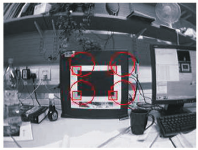
\includegraphics[height=6.0cm]{img/cap4/Initialization4PointsMonoSlam.png}}
\end{center}
\caption{Inicialización de MonoSLAM con 4 puntos conocidos.}
\end{figure}

El EKF, tiene un vector de estado compuesto de posición, orientación y velocidad de la cámara y además las coordenadas 3D de los puntos conocidos en un cierto momento, esto implica que el vector de estado irá aumentando de tamaño a medida que vayamos descubriendo nuevos puntos 3D. El modelo de observación estará compuesto de las proyecciones de cada uno de los puntos 3D en el plano imagen.

El uso de un EKF es apropiado, ya que se realizan iteraciones cada pocos milisegundos, y por tanto en intervalos de tiempo tan pequeños, el sistema puede aproximarse a un sistema lineal. Cuantas más iteraciones o frecuencia de muestreo la estimación mejora. En cada iteración se hace una detección de puntos de interés (esquinas con FAST) en la imagen actual de entrada, y obtendremos una serie de puntos que serán candidatos a ser el vector observación de los puntos que queremos seguir. Estos candidatos deberán ser filtrados, pues alguno puede ser un falsa esquina. Se utilizará una función de divergencia ZMSSD (\textit{Zero Mean Sum of Squared Differences}) entre parches para determinar si el candidato es aceptable o no. Al utilizar sólo parches de unos pocos píxeles alrededor del candidato, estamos optimizando el computo ya que no requiere procesar toda la imagen.

Aún así es posible que se acepten puntos candidatos que no sean apropiados. Para tratar de eliminar estos falsos positivos, \cite{civera20101} propuso una alternativa conocida como 1-Point RANSAC.
MonoSLAM es recomendable para mapas con pocos puntos. Es muy sensible a movimientos bruscos y por tanto difícilmente podrá recuperarse de un secuestro. Si la hipótesis de partida no es correcta el filtro podría desestabilizarse y no llegar nunca a aproximar razonablemente el vector de estado.


%\begin{figure}[htbp]
\begin{figure}[H]
\begin{center}
\subfigure[]{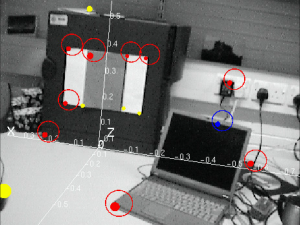
\includegraphics[height=5.0cm]{img/cap4/monoslam-300x225.png}}
\end{center}
\caption{Ejemplo de puntos característicos tomados con MonoSLAM.}
\end{figure}
\clearpage


\subsection{PTAM}
\textit{Parallel Tracking and \textit{Mapping}}. Es un algoritmo creado en 2007 por George Klein \cite{Klein2007parallel} que también calcula el Tracking y el \textit{Mapping} como en MonoSLAM pero para ello utiliza 2 \textit{Threads}, uno para calcular el posicionamiento de la cámara (Tracking ) y el segundo para la generación del mapa (\textit{Mapping}). Esta separación en dos hilos de ejecución se debe a que el Tracking necesita ser calculado en tiempo real para obtener una localización precisa, mientras que el \textit{Mapping} puede demorarse más tiempo sin perjudicar a la localización de la cámara. 

Con las imágenes captadas en secuencia se van generando \textit{Keyframes} o fotogramas clave. Se genera un nuevo \textit{Keyframe} a medida que la cámara se va desplazando. Los \textit{Keyframes} se utilizan para la localización y para ir generando el mapa de puntos.
Este algoritmo es recomendable para mapas con elevado número de puntos, es capaz de recuperarse fácilmente de un secuestro, extrae los puntos de interés mediante extracción de características como en MonoSLAM y trata de emparejarlos con los puntos extraídos de las imágenes anteriores.  Como extractor de características utiliza el detector FAST. Se realizará una subdivisión de la imagen a distintas resoluciones, normalmente 4 niveles, lo que se conoce como pirámide de la imagen y se pasará un filtro FAST sobre esta pirámide para detectar los puntos más característicos de la imagen.
Cada \textit{Keyframe} que se genera, contiene  la imagen captada junto su pirámide y sus puntos de interés detectados. Cuando añadimos un \textit{Keyframe}, se intenta localizar en este \textit{Keyframe} los puntos que ya se encuentran en el mapa, en caso de no ĺlocalizarlos se añaden nuevos puntos al mapa. Mientras no se añadan \textit{Keyframes}, se intentará mejorar el mapa con los \textit{Keyframes} disponibles optimizando con Bundle Adjustment.

Se suele utilizar en entornos cerrados y pequeños y utiliza técnicas SFM. Muy utilizado también para realidad aumentada.

%\begin{figure}[htbp]
\begin{figure}[H]
\begin{center}
\subfigure[]{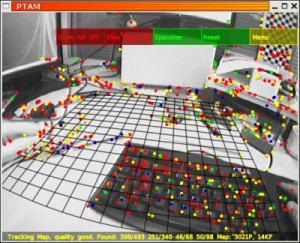
\includegraphics[height=6.0cm]{img/cap4/ptam_screenshot-300x243.jpg}}
\end{center}
\caption{Nube de puntos característicos tomados con PTAM.}
\end{figure}



\clearpage

\subsection{ORB-SLAM}
Es un algoritmo basado en extracción y emparejamiento de píxeles característicos mediante descriptores ORB, estos descriptores son más fiables que los parches tradicionales y por tanto permiten obtener mapas robustos y precisos tanto en escenarios de grandes dimensiones como en zonas pequeñas, sin embargo para su funcionamiento en tiempo real requiere la utilización de ordenadores con alta capacidad de proceso \cite{Mur2015orb}.
Puede ser utilizado con una cámara o dos e incluso con cámaras de profundidad RGBD. Para cierres de bucle y relocalización utiliza un modelo de bolsa de palabras \cite{galvez2012bags}.
Utiliza 3 \textit{Threads}, el primero para Tracking, el segundo para \textit{Mapping} y un tercero para detectar cierres de bucle. 

En el proceso de Tracking, se trata de calcular la posición actual a partir de los emparejamientos encontrados de los puntos 3D en el fotograma anterior, para ello utilizará los descriptores ORB.
En caso de perdida, el robot podrá relocalizarse gracias a un modelo de bolsa de palabras que le permitirá encontrar \textit{Keyframes} candidatos que concuerden con la observación actual (Figura \ref{fig:ORBMatching}).

En el proceso de \textit{Mapping}, se inicializarán 2 mapas, uno por homografía y el segundo mediante una matriz fundamental. Los 2 mapas recibirán una puntuación y se elegirá como candidato para inicializar el mapa aquel que obtenga mayor puntuación. Cuando ya se dispone del mapa inicial, se procesan los \textit{Keyframes} creando nuevos puntos 3D y se optimiza localmente el mapa mediante Bundle Adjustment. A su vez se genera un grafo donde cada \textit{Keyframe} se corresponde con un vértice y un vértice estará unido a otro siempre y cuando los \textit{Keyframe} tengan varios puntos 3D en común. Este grafo permite la eliminación de \textit{Keyframe} redundantes (Figura \ref{fig:ORB_SLAM}).

En el proceso de Looping, se comprobará si se ha producido un cierre de bucle. Utilizando el grafo de \textit{Keyframe} conectados y el modelo de bolsa de palabras se intenta encontrar \textit{Keyframe} candidatos que tengan una apariencia similar a la imagen actual.

%\begin{figure}[htbp]
\begin{figure}[H]
\begin{center}
\subfigure[]{\label{fig:ORBMatching}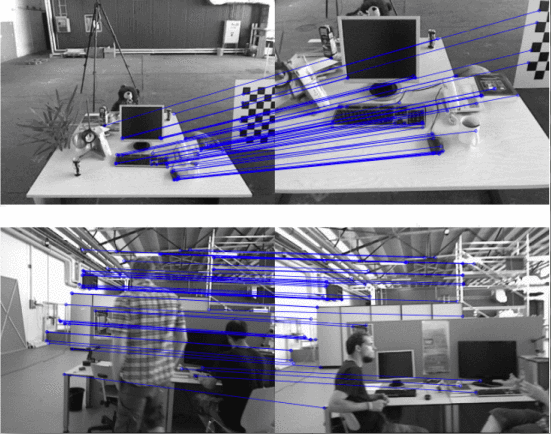
\includegraphics[height=5.5cm]{img/cap4/ORB_localization.png}}
\hspace{0.5cm}
\subfigure[]{\label{fig:ORB_SLAM}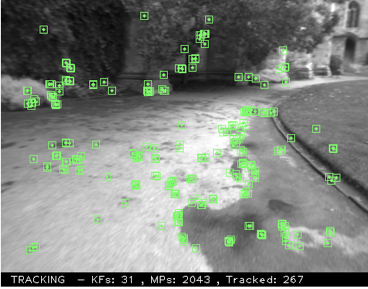
\includegraphics[height=5.5cm]{img/cap4/ORB_SLAM.png}}
\end{center}
\caption{Localización de puntos característicos en 2 imágenes con ORB }
\end{figure}

\clearpage

\subsection{DSO y LDSO}
\textit{DSO: Direct Sparse Model}.
Está basado en optimizaciones continuas del error fotométrico sobre una ventana de frames recientes\cite{Engel2016direct}.
El inicio del Tracking, cuando se crea un nuevo \textit{Keyframe}, todos los puntos activos son proyectados en el y ligeramente dilatados, creando así un mapa de profundidad semi denso. Nuevos frames son creados con respecto a este frame utilizando alineamiento directo de 2 frames, una pirámide multi escala y un modelo de movimiento constante a inicializar. 
Para la relocalización, se podrán trazar hasta 27 rotaciones pequeñas en diferentes direcciones. Esta recuperación de posición se consigue en el nivel más pequeño de la pirámide de la imagen.
La creación de \textit{Keyframes} es similar a ORB-SLAM, existen 3 criterios para determinar cuando se necesita un nuevo \textit{Keyframe}.
\begin {enumerate}
\item Se creará un nuevo \textit{Keyframe} (Figura \ref{fig:mapaDSO}) cuando la imagen de entrada cambie notablemente con respecto al último \textit{Keyframe}, esto se medirá con la diferencias de medias al cuadrado entre los píxeles.
\item La traslación de la cámara causa oclusiones y des-oclusiones, lo cual indica que se deben generar nuevos \textit{Keyframes}
\item Si el tiempo de exposición de la cámara cambia significativamente, se deberá tomar un nuevo \textit{Keyframe}. Esto se mide por el factor de brillo relativo entre 2 frames. 
\end {enumerate}

En cuanto al rechazo de \textit{Keyframes}, sigue la siguiente estrategia. Sean $I_1$ \dots $I_n$ un conjunto de \textit{Keyframes} activos, siendo $I_1$ el más nuevo y $I_n$ el más antiguo
\begin {enumerate}
\item Siempre se mantendrán los dos últimos \textit{Keyframes} ($I_1$  e $I_2$ )
\item Frames con menos del 5\% de sus puntos visibles en $I_1$  son descartados.
\item Si mas de N frames están activos, se descartan (exceptuando $I_1$  e $I_2$) aquel que maximice un marcador de distancia d(i,j) donde d(i,j) es la distancia Euclídea entre \textit{Keyframes} $I_1$  e $I_j$
\end {enumerate}

Sobre el tratamiento de los puntos, siempre se tratará de mantener un numero fijo de puntos activos repartidos de forma uniforme entre el espacio y los frames activos. En un primer paso, se identifican Np puntos candidatos en cada nuevo \textit{Keyframe}. Los puntos candidatos no son inmediatamente sumados a la optimización, sino que son localizados individualmente en sucesivos frames generando una primera estimación del valor de profundidad que servirá como inicialización. 

En cuanto a la selección de puntos candidatos, se intentará seleccionar aquellos puntos que están bien distribuidos en la imagen y tienen un valor elevado de gradiente con respecto a sus alrededores. Para obtener una distribución uniforme de puntos sobre la imagen, esta se divide en bloques de $dxd$, de cada bloque se elegirá el píxel con el mayor gradiente siempre y cuando supere un umbral, de lo contrario no se selecciona el píxel de ese bloque. Los puntos candidatos son localizados en siguientes frames utilizando una búsqueda sobre la línea epipolar minimizando el error fotométrico. Una vez hallamos encontrado las coincidencias preparamos un valor de profundidad y la varianza asociada que se utilizará para restringir el intervalo de búsqueda en frames siguientes. Esta estrategia de localización está inspirada en LSD-SLAM.

Por último, la activación de puntos candidatos, cuando un conjunto de puntos antiguos son marginados, nuevos puntos candidatos son activados para remplazarlos, siempre intentando mantener una distribución uniforme de puntos por toda la imagen \footnote{https://ieeexplore.ieee.org/stamp/stamp.jsp?arnumber=7898369}.

%\begin{figure}[htbp]
\begin{figure}[H]
\begin{center}
\subfigure[]{\label{fig:mapaDSO}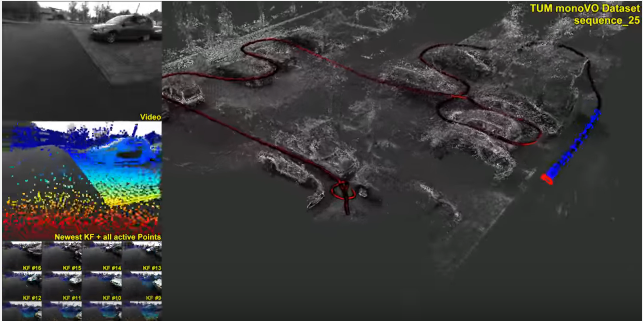
\includegraphics[height=6.0cm]{img/cap4/mapaDSO.png}}
\hspace{0.5cm}
\subfigure[]{\label{fig:fotogramaDSO}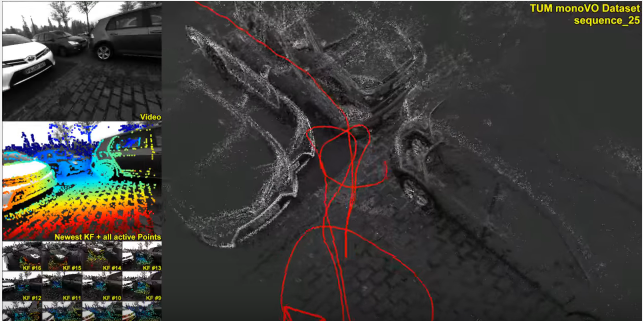
\includegraphics[height=6.0cm]{img/cap4/fotogramaDSO.png}}
\end{center}
\caption{Mapa generado con DSO (a) Ligero error en la posición al volver al punto de partida (b).}
\end{figure}

\clearpage

\textit{LDSO: Direct Sparse Odometry with Loop Closure}. Este método es una extensión del algoritmo DSO (Direct Sparse Odometry). LDSO incorpora detección de cierre de bucle y optimización de posición y mapeo. Al ser un método directo, DSO puede utilizar cualquier pixel de la imagen con suficiente gradiente de intensidad, lo cual lo hace más robusto incluso en áreas donde apenas se pueden obtener puntos característicos. LDSO mantiene esta robusted, mientras que al mismo tiempo asegura la repetibilidad  sobre alguno de esos puntos prestando más atención sobre esquinas características en el proceso de tracking. Estas repetibilidad de puntos característicos permite detectar de forma fiable los candidatos de cierres de bucle utilizando la técnica basada en carácterísticas de bag-of-words. 
Los candidatos a cierre de bucle son verificados geométricamente y restricciones de pose relativa son estimadas minizando en conjunto errores geométricos 2D y 3D.
Selección de puntos de características Repetibles, DSO utiliza un grid dinamico para detectar suficientes pixels incluso en entornos con pocas texturas. Más especificamente, todavía se toma un numero determinado de pixeles ( por defecto 2000 en DSO), de los cuales algunos son esquinas. Manteniendo el número de esquinas pequeño se calculan los descriptores ORB y los empaquetamos en BoW. El algoritmo  utiliza ambos tipos de pixeles de esquinas y no esquinas para obtener el tracking, y la carga del thread para obtener el cierre de bucle permanece al mínimo.
En un frame capturado mediante DSO hay pocos elementos repetibles y por tanto es dificil buscar emparejamiento de imágenes usando esos puntos para cierre bucle. Pero en LDSO se utilizan ambos esquinas y otros pixeles con alto gradiente, donde las esquinas se utilizan para construir modelos BoW (Bag of Words) y para tracking, mientras que los no esquinas sólo se utilizan para tracking. De esta forma podemos hallar la posición en entornos con pocas texturas y tambien encontrar caracteristicas comunes entre keyframes si lo necesitasemos.
Cada vez que calculamos descriptores ORB para cada keyframe, una base de datos BoW es construida. Los candidatos a cierre de bucle son propuestos para el keyframe actual mediante consultas a la base de datos y solo se toman aquellos que están fuera de la actual ventana. Para cada candidato intentamos machear sus características ORB a aquellos del keyframe actual, y entonces ejecutamos RANSAC PnP para computarla estimación inicial de la transformación. Despues se optimiza la transformación usando el método de Gauss-Newton mediante la minimización de restricciones geométricas 3D y 2D.
\begin{figure}[H]
\begin{center}
\subfigure[]{\label{fig:LDSO}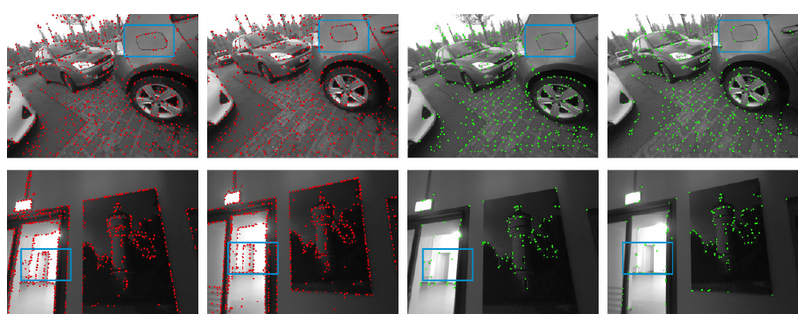
\includegraphics[height=6.0cm]{img/cap4/LDSO.png}}
\end{center}
\caption{diferencias entre puntos escogidos con DSO y LDSO.}
\end{figure}


\section{Herramientas para realizar evaluaciones comparativas de algoritmos SLAM}
En este apartado trataremos sobre varias herramientas que podemos utilizar para hacer benchmarking sobre los resultados de algoritmos SLAM y evaluar y comparar dichos resultados

\begin {enumerate}
%\subsection{Computer Vision Group TUM}
\item\textbf{Computer Vision Group TUM}

Proporciona varias herramientas para evaluar el rendimiento de algoritmos VSLAM, permite evaluar trayectorias y compararlas con la trayectoria ground truth.\cite{sturm12iros}
Utiliza principalmente 2 métodos, el error absoluto de la trayectoria \textit{absolute trajectory error (ATE)} y el error relativo a la posición \textit{relative pose error (RPE)}. Podemos encontrar en la web HERE scripts descargables para ambas métricas.

Las trayectorias que vayan a ser evaluadas deben ser almacenadas en un archivo de texto, donde cada línea contendrá una única posición con el siguiente formato( 'timestamp tx ty tz qx qy qz qw')

Donde el campo timestamp, tipo float proporciona el número de segundos , tx ty tz que son de tipo float, dan la posición del centro óptico de la cámara con respecto al origen de coordenadas del mundo real , qx qy qz qw , también de tipo float, dan la orientación del centro óptico de la cámara  con respecto al origen de coordenadas del mundo real pero en formato de quaternio unidad.


%\begin {enumerate}
%\item \textbf{Absolute Trajectory Error (ATE)}
 \textbf{\textit{Absolute Trajectory Error (ATE)}}:
 El error absoluto de trayectoria mide la diferencia que existe entre cada punto de la trayectoria estimada y la trayectoria real. Como paso de preproceso se realiza una asociación entre la posición estimada con la posición ground truth utilizando el emparejamiento por timestamps o marcas de tiempo. Tras esta asociación, se alinea la trayectoria real con la estimada usando SVD (Singular Value Decomposition). Por último, el ordenador calula la diferencia entre cada par de posiciones y devuelve valores estadísticos como la media,mediana y desviación estandar de estas diferencias. También es posible obtener gráficos con las 2 trayectorias.

%\item \textbf{Relative Pose Error (RPE)}
\textbf{\textit{Relative Pose Error (RPE)}}: 
Con el script python evaluaterpe.py es posible calcular el error relativo a la posición . Este script obtiene el error entre el movimiento relativo entre pares de timestamps. Por defecto el script calcula el error entre todos los pares de timestamps del fichero de trayectoria. Como el numero de pares de timestamps en la trayectoria estimada es cuadrático se pueden poner cotas con un número máximo de pares de timestamps. Opcionalmente, tambien se puede elegir usar un tamaño de ventana ficho (-fixed delta). En este caso cada pose en la trayectoria estimada es asociado con posteriores posiciones dependiendo del tamaño de ventana (-delta) y unidad (-delta unit). Esta técnica de evaluación es util para calcular el desvio o deriva.



%\end {enumerate}


\item \textbf{Trajectory Evaluation Toolbox for Visual(-inertial) Odometry}

Esta herramienta está desarrolla en python e incluye : 
Métodos de alineamiento de trayectorias para diferentes modalidades de sensores
Métricas de error tales como ATE y Relative Odometry Error. \cite{Zhang18iros}

El software ha sido diseñado para uso facil. Dados 2 ficheros de texto donde especificaremos la trayectoria estimada y el groundtruth, la herramienta establece automáticamente el emparejamiento de tiempos, realiza alineamiento de trayectoria y calcula distintos errores métricos con una línea de comandos. Tambien se puede utilizar para comparar diferentes algoritmos con múltiples datasets. Para que la aplicación pudiese ser utilizada con diferentes formatos, tambien se proporcionan varios scripts para convertir otros formatos conocidos (e.g., EuRoC, rosbag) al formato utilizado por la herramienta.
El formato utilizado para los ficheros de datos es el siguiente: timestamp tx ty tz qx qy qz qw

\item \textbf{SLAMBENCH}

SLAMBench es una herramienta de la Universidad de Edimburgo, esta herramienta ha sido creada para evaluar sistemas SLAM ya sean sistemas de código abierto o sistemas propietarios sobre un conjunto extensible de datasets y métricas. \cite{Bodin2018}
Actualmente soporta 8 tipos distintos de algoritmos (densos, semi-densos y escasos ) y 3 datasets. Es una herramienta que permite la reproductibilidad de los resultados para los sistemas SLAM actuales y posibilita la integración y evaluación the nuevos resultados SLAM.

SLAMBench soporta varios algoritmos diferentes. Entre los algoritmos escasos o poco densos soportaría los siguientes MonoSLAM, PTAM ,OKVIS y ORB-SLAM2. Los 2 primeros algoritmos soportan solo sistemas monoculares, OKVIS soporta sólo estereo y RGB-D y ORBSLAM2 soporta ambos tipos. Estos algoritmos son algoritmos indirectos.
Entre los métodos densos se soportan 3 tipos de algoritmos, KinectFusion, InfiniTAM, ElasticFusion que son 2 recientes modelos densos. Por último LSD-SLAM es un sistema SLAM semi-denso de una sola cámara (monocular).
\begin{figure}[H]
\begin{center}
\subfigure[]{\label{fig:LDSO}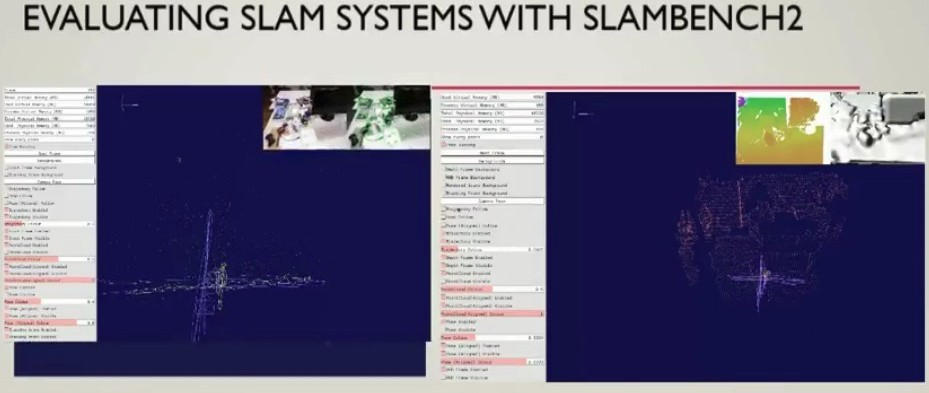
\includegraphics[height=6.0cm]{img/cap4/slambench.jpg}}
\end{center}
\caption{captura de la herramienta SLAMBENCH2.}
\end{figure}

Para medir el rendimiento de algoritmos SLAM se puede utilizar un framework para cuantificar la calidad de los resultados teniendo en cuenta exactitud, tiempo de ejecución, uso de memoria y consumo de energía. Esta información puede ser visualizada gracias a su interfaz gráfico.
Además SLAMBench ofrece una plataforma con grandes posibilidades para investigaciones futuras ya sea para diseño de algoritmos como optimizaciones a nivel de implementación. Es una herramienta multiplataforma y se puede utilizar en PCs de sobremesa, portátiles y móbiles. Algunos benchmarks se han obtenido con Ubuntu, OS y Android.
También puede ser utilizado con CUDA.
SLAMBench proporciona, entre otras métricas, medidas de exactitud del algoritmo utilizado. Las medidas de exactitud son determinadas comparando datos estimados con los datos ground-truth.
Absolute Trajectory Error (ATE) y Relative Pose Error RPE son utilizadas para medir la exactitud de la trayectoria. Estas métricas de trayectoria junto con una métrica de mapeo, Reconstruccion de Error , proporcionan comparaciones cuantitativas para varios algoritmos.

ATE y RPE son calculadas en tiempo de ejecución, con un alineamiento mínimo entre la primera posición más cercana de ground-truth y la posición estimada ( en términos de timestamp). Ya off-line, técnicas más complejas de alineamiento pueden ser usadas para comparar técnicas densas y semidensas cuando el mapeo de escalas no funciona. RER se calcula mediante la ejecución del algoritmo Iterative Closest Point (ICP) de los modelos de la nube de puntos de la reconstruncción y del ground truth. Como este proceso consume mucha CPU esta evaluación es tambien ejecutada off-line.

Otras métricas que proporciona SLAMBench es el consumo de energía ,utilización de memoria, velocidad de proceso por frame.

Interface de usuario modular: SLAMBench tambien permite elegir entre diferentes sistemas de interfaz de usuario. Métricas de evaluación pueden ser cambiadas y customizadas, así como el interfaz de usuario gráfico (GUI), mientras mantiene independencia de los datasets y algoritmos. Por ejemplo, el visualizador nativo está basado en la librería Pangolin , puede ser reemplazado por un visualizador ROS.

SLAMBench está siendo un componente muy importante en robótica y Sistemas de Realidad Aumentada (AR). Aunque un gran número de algoritmos SLAM han sido presentados, no se ha investigado lo suficente para tratar de unificar el interface de estos algoritmos, o realizar comparaciones de todas sus capacidades en conjunto. Esto presenta un problema ya que diferentes aplicaciones SLAM pueden tener diferentes requisitos funcionales y no funcionales. Por ejemplo, una solución para Realidad Aumentada desarrollada para móviles tendría que optimizar el consumo de energía, mientras que otra solución diseñada para vehículos de navegación autónoma estaría enfocada a funcionar con la mayor exactitud posible. SLAMBench2 es un framework de evaluación que compararía sistemas SLAM actuales y futuros, utilizando una lista extensible de datasets, mientras utiliza una lista comparable de métricas de rendimiento. Se podrían utilizar una gran variedad de algoritmos de SLAM y datasets como ElasticFusion, ORB-SLAM2, OKVIS y tambien se podría integrar con nuevos algoritmos y datasets. SLAMBench2 es un software que está disponible de manera pública. 

\item \textbf{The Kitti Vision Benchmark Suite }

Es un conjunto de aplicativos que utilizan mapas y secuencias grabados desde la plataforma de coches autónomos Annieway para crear nuevos desafíos o retos en las tareas comparativas o benchmarking de visualslam.\cite{Geiger2012CVPR}
Están investigando en varios campos como: vision stereo, flujo optico, odometría, detección de objetos en 3D y seguimiento de objetos 3D.
La exactitud de los conjuntos de datos ground truth es medida gracias al scanner laser Velodyne y a los sistemas de localización GPS con los que van equipados sus coches autónomos.
Los datasets han sido grabados en la ciudad de Karslruhe.
Además de proporcionar todos los datos en formato raw, para cada uno de sus benchmarks, también proporcionan una metrica de evaluación y una web de evaluación de métricas. En experimientos preliminares se ha comprobado que métodos que obtienen una puntuación alta en algunos benchmarks, cuando son aplicados al mundo real obtienen unos resultados por debajo de la media. El objetivo es reducir esta tendencia y completar los benchmarks existentes proporcionando benchmarks en el mundo real con dificultades novedosas para la comunidad. 

Un ejemplo podría ser el benchmark de odometría, que consiste en 22 sequencias stereo, grabadas en formato png. En el dataset se proporcionan 11 secuencias con trayectorias ground truth para entrenar y 11 sequencias sin ground truth para evaluar. Para este benchmark se pueden proporcionar reusltados usando una cámara o un sistema de cámaras estereo.
La única restricción que se impone es que el metodo deber ser totalmente automático (no se permite el etiquetado manual de cierre de bucle) y que el mismo conjunto de parámetros es usado para todas las secuencias.
Para todas las secuencias de test, su evaluador estima los errores de traslación y rotación. En una tabla de evaluación se establece un ranking de métodos de acuerdo con la media de esos valores, donde los errores son medidos en porcentaje para la trasalación y en grados por metro para la rotación.
\begin{figure}[H]
\begin{center}
\subfigure[]{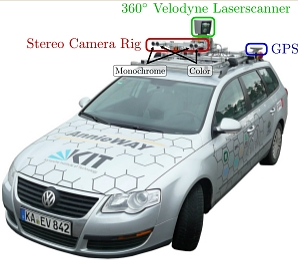
\includegraphics[height=6.0cm]{img/cap4/kittiCar.png}}
\end{center}
\caption{Coche autónomo Annieway utlizado con Kitti.}
\end{figure}

\end {enumerate}


\section{Comparativa de los algoritmos más representativos} 
A continuación se presenta una tabla que muestra las características principales de cada algoritmo. Esta tabla es similar a la que aparece en \cite{Perdices17} pero en este caso se ha añadido el algoritmo DSO.

\begin{center}
% \begin{tabular}{||c c c c c c c c||} 
\begin{tabular}{ |m{2.5cm} | m {1.5cm}| m {1.7cm}| m {1.7cm} | m {1.7cm}| m {1.7cm}| m {1.7cm}| m {1.7cm}| }
 \hline
 Funcionalidad & Mono-SLAM & PTAM & ORB-SLAM & LDSO  \\ [0.5ex] 
 \hline\hline
 Probabilístico & Sí & No & No & No \\ 
 \hline
 Hilos de ejecución & 1 & 2 & 3 & 2\\
 \hline
 Emparejamien-to & Parches & Parches & ORB & Métodos directos \\
 \hline
 Puntos 3D con incertidumbre & No & No & No & Sí\\
 \hline
 Mapa inicial & Dado & Homograf. & Homog. /Matriz F. & Incerti-dumbre \\ [1ex] 
 \hline
 \textit{Keyframes} & No & Sí & Sí & Sí  \\ [1ex] 
 \hline
 Puntos en mapa & Cientos & Miles & Miles & Miles \\ [1ex] 
 \hline
 Mapa denso & No & No & No & Semi-denso\\ [1ex] 
 \hline
 Gestión de mapas grandes & No & No & Sí & Sí \\ [1ex] 
 \hline
 Relocalización & No & Sí & Sí & No\\ [1ex] 
 \hline
 Rechazos de espurios & No & No & Sí & No\\ [1ex] 
 \hline
 Cierre de bucle & No & No & Sí & Sí\\ [1ex] 
 \hline
\end{tabular}
\end{center}
\clearpage
%\flushbottom
\newpage
\pagebreak










